% This is samplepaper.tex, a sample chapter demonstrating the
% LLNCS macro package for Springer Computer Science proceedings;
% Version 2.21 of 2022/01/12
%
\documentclass[runningheads]{llncs}
%
\usepackage[T1]{fontenc}
% T1 fonts will be used to generate the final print and online PDFs,
% so please use T1 fonts in your manuscript whenever possible.
% Other font encondings may result in incorrect characters.
%
\usepackage{graphicx}
% Used for displaying a sample figure. If possible, figure files should
% be included in EPS format.
%
% If you use the hyperref package, please uncomment the following two lines
% to display URLs in blue roman font according to Springer's eBook style:
%\usepackage{color}
%\renewcommand\UrlFont{\color{blue}\rmfamily}
%
\usepackage{tikz, wrapfig}

\begin{document}
%
\title{Active Automata Learning of an IPsec IKEv1 Server using AALpy}
%
%\titlerunning{Abbreviated paper title}
% If the paper title is too long for the running head, you can set
% an abbreviated paper title here
%
\author{Benjamin Wunderling\inst{1}\orcidID{0000-1111-2222-3333}}

%
\authorrunning{Benjamin Wunderling}
% First names are abbreviated in the running head.
% If there are more than two authors, 'et al.' is used.
%
\institute{TU Graz IST, Graz 8010, Austria \\
\email{benjamin.wunderling@student.tugraz.at}}
%
\maketitle              % typeset the header of the contribution
%
\begin{abstract}
Virtual Private Network (VPN) protocols are widely used to create a secure mode of communication between several parties over an insecure channel. A common use-case for VPNs is to secure access to company networks. Therefore errors in VPN software are often severe. IPsec is a VPN protocol that uses the Internet Key Exchange protocol (IKE). IKE has two versions, IKEv1 and the newer IKEv2. While several papers have investigated IPsec-IKEv2 in the context of Automata learning, no such work has been performed for IPsec-IKEv1. This short paper describes the IPsec-IKEv1 protocol and show the steps taken to learn the state-machine of an IPsec server. We present a learned model and discuss its potential applications for model-based fuzzing and fingerprinting of IPsec implementations.

\keywords{IPsec  \and Automata Learning \and AALpy.}
\end{abstract}
%
%
%
\section{Introduction}
% background
VPNs are used to allow secure communication over an insecure channel. The importance of VPN software has increased dramatically since the beginning of the COVID-19 pandemic due to the influx of people working from home \cite{abhijith2020impact}. This makes finding vulnerabilities in VPN software more critical than ever. IPsec is a VPN protocol and most commonly uses the IKE protocol to share authenticated keying material between involved parties. Therefore, IKE and IPsec are sometimes used interchangeably. We will stick to the official nomenclature of using IPsec for the full protocol and IKE for the key exchange only. IKE has two versions, IKEv1 IKEv2, with IKEv2 being the newer and recommended version \cite{nist791491}. However, despite IKEv2 supposedly replacing its predecessor, IKEv1 is still in widespread use today. This is reflected by the company AVM to this day only offering IKEv1 support for their popular Fritzbox routers \cite{avm2022}.

%Problem
State models of protocol implementations are useful tools in testing. They can for example be used to detect software versions \cite{pferscher2021fingerprinting}, or generate test cases automatically \cite{pferscher2022fuzzing}. One method of generating such models is to use Active Automata Learning. A notable example of an Active Automata Learning algorithm is the L* algorithm by Angluin \cite{angluin1987learning}. In L*, a teacher queries the System under Learning (SUL) and through its responses can construct an automaton describing the behavior of the SUL. This automaton can then be compared with the SUL, adapting it if they show different behaviors. Several papers have investigated IPsec-IKEv2 using Automata Learning, however so far none have looked at IKEv1. 

% My solution
We show the process of learning a state model from an example IPsec-IKEv1 server. We use the Active Automata Learning framework AALpy \cite{muvskardin2022aalpy} for L* Automata Learning, with a custom Python interface between AALpy and the IPsec server.

% Structure of Thesis
In this short paper we first go over preliminary information on VPNs and Automata Learning in chapter \ref{chap:2}. In \ref{chap:3} we discuss other related work. In chapter \ref{chap:4} we briefly introduce AALpy and our learning setup. Then we will present our custom interface between AALpy an the IPsec server, discussing design choices and implementation difficulties. Finally we present the learned model and discuss its potential applications and further work in chapters \ref{chap:5} and \ref{chap:6}.



\section{Preliminaries} \label{chap:2} % 1 page
\subsection{Automata Learning}
% More on Automata Learning, in particular L*
Automata Learning refers to methods of learning a state model, or automata, of a system through an algorithm or process. We differentiate between Active and Passive Automata Learning. In Passive Automata Learning (PAL), models are learned based on collected logs or other information describing the behavior of the system under learning (SUL). In contrast, in Active Automata Learning (AAL) the SUL is queried directly. In this short paper, we will focus on AAL and will moving on refer to it as Automata Learning or AAL interchangeably. 

AAL began in 1987 with a paper by Dana Angluin, titled "Learning regular sets from queries and counterexamples"\cite{ANGLUIN198787}. In this seminal paper, Dana introduced the L* algorithm which is still used for learning deterministic automata. L* works using a Minimally Adequate Teacher (MAT) model in which a learner queries a teacher about a SUL. The teacher must be able to answer equivalence and membership queries posed by the learner regarding the SUL. Equivalence queries are used to check if a learned model accurately matches the SUL and membership queries are used to check how the SUL reacts to a particular input. The learner, using the responses to its queries, then updates its model of the SUL. Learned models are commonly represented as Mealy machines, finite-state machines with outputs depending on the current state as well as external inputs. % in actual paper, a full definition will be given of both L* and Mealy machines.

\subsection{IPsec}
% More on VPNs, in particular about IPsec
IPsec or IP Security, is a VPN layer 3 protocol used to securely communicate over an insecure channel. It is based on three sub-protocols, IKE, the Authentication Header protocol (AH) and the Encapsulating Security Payload protocol (ESP). IKE is mainly used to handle authentication and to securely exchange and manage keys. Following a successful IKE round, either AH or ESP is used to send packets securely between parties. The main difference between AH and ESP is that AH only ensures the integrity and authenticity of messages while ESP also ensures the confidentiality through encryption.
Compared to other protocols, IPsec offers a high degree of customizability, allowing it to be fitted for many use-cases. However, in a cryptographic evaluation of the protocol, Niels Ferguson and Bruce Schneier criticized that customizability stating that the biggest weakness of IPsec is its complexity \cite{ferguson1999cryptographic}. To address its main criticism IPsec-IKEv2 was introduced in RFC 7296 to replace IKEv1 \cite{kaufman2014internet}. Regardless, IPsec-IKEv1 is still in wide-spread use to this day, with the largest router producer in Germany AVM still only supporting IKEv1 in their routers \cite{avm2022}. We use IPsec-IKEv1 with ESP and main mode in this short paper and focus on the IKE protocol as it is the most interesting from an AAL and security standpoint. % this part could maybe be moved to the introduction, not sure

\begin{wrapfigure}{1}{0pt}
	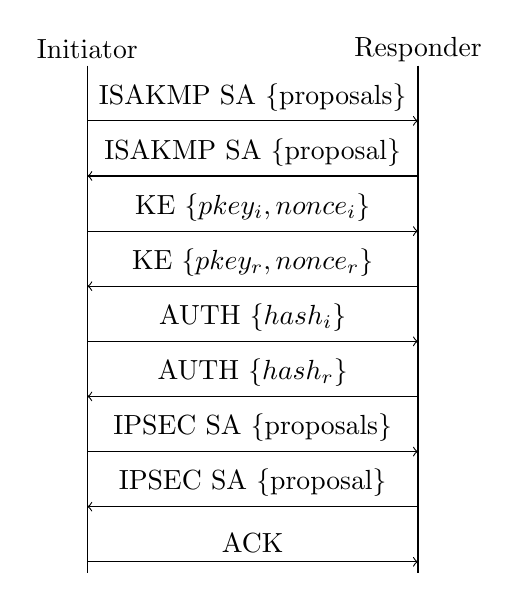
\begin{tikzpicture}[scale=0.7]
	\draw (-3,0) -- (-3,-9.2) (3,0) -- (3,-9.2);
	\node at (-3,.3) {Initiator};
	\node at (3,.3) {Responder};
	\draw[->] (-3,-1) -- node[midway,above] {ISAKMP SA \{proposals\}} (3,-1);
	\draw[<-] (-3,-2) -- node[midway,above] {ISAKMP SA \{proposal\}} (3,-2);
	\draw[->] (-3,-3) -- node[midway,above] {KE $\{pkey_i, nonce_i\}$} (3,-3);
	\draw[<-] (-3,-4) -- node[midway,above] {KE $\{pkey_r, nonce_r\}$} (3,-4);
	\draw[->] (-3,-5) -- node[midway,above] {AUTH $\{hash_i\}$} (3,-5);
	\draw[<-] (-3,-6) -- node[midway,above] {AUTH $\{hash_r\}$} (3,-6);
	\draw[->] (-3,-7) -- node[midway,above] {IPSEC SA \{proposals\}} (3,-7);
	\draw[<-] (-3,-8) -- node[midway,above] {IPSEC SA \{proposal\}} (3,-8);
	\draw[->] (-3,-9) -- node[midway,above] {ACK} (3,-9);
	\end{tikzpicture}
	\caption{IKEv1 between two parties}
	\label{fig:IKEv1}
\end{wrapfigure}

The IKEv1 protocol works in two main phases, both relying on the Internet Security Association and Key Management Protocol (ISAKMP) protocol. A typical exchange between two parties can be seen in figure \ref{fig:IKEv1}. Assuming two participants, an initiator and a responder, in phase one (Main Mode) the initiator sends a Security Association (SA) to the responder. A SA essentially details important security attributes for a connection like the encryption algorithm and key-size to use, as well as the authentication method and the used hash algorithm. These options are bundled in containers called proposals, with each proposal describing a possible security configuration. While the initiator can send multiple proposals to give the responder more options to choose from, the responder must answer with only one, provided it supports one of the suggested proposals. Next, the two parties perform a Diffie-Hellman key exchange and exchange nonces to generate a shared secret key. This secret key is used as a seed key for all further session keys. Following a successful key exchange, all further messages are encrypted. Finally, both parties exchange hashed authentication material (usually pre-shared keys or certificates) and verify the received hash. If successful, a secure channel is created and is used for phase two communication.
The shorter phase two (Quick Mode) begins with another SA exchange, this time however the SA describes the security parameters of the ensuing ESP/AH communication. This is followed by a single acknowledge message from the initiator to confirming the agreed upon proposal. After the acknowledgment, all further communication is done via ESP/AH packets. 


\section{Related Work} \label{chap:3} % 1/2 page
% Discuss related papers (chinese, other similar protocols?)
Model learning of other network protocols like SSH \cite{fiteruau2017model}, or TCP \cite{fiteruau2016combining} has been performed in the past, with learned model being used for model checking the learned protocols. Both \cite{novickis2016protocol} and \cite{daniel2018inferring} learned models of the more related OpenVPN protocol \cite{novickis2016protocol} and used the learned models for fuzzing. In \cite{pferscher2021fingerprinting}, learned models were used to fingerprint Bluetooth Low Energy Devices. Guo et al. used Automata Learning to learn and test the IPsec-IKEv2 protocol \cite{guo2019model}. However, they used the LearnLib library to learn their automata and used the learned model for model checking. No fuzzing or fingerprinting was performed. Our goal is to in future work use the learned model for either fuzzing or to fingerprint different IPsec implementations.


\section{Learning IPsec} \label{chap:4} %or other title --> method, eihter way, decribe design decisions here ~1.5 pages
\subsection{Setup} % 1/2 page
% describe VMs, IPsec server software, configuration etc
We developed and tested our interface using two Virtual Box virtual machines (VMs) running standard Ubuntu distributions. All communication took place in an isolated virtual network to eliminate possible external influences. We designated one VM as the initiator and one as the responder to model a typical client server setup. The open source IPsec implementation Strongswan was installed on the responder VM and set to listen for incoming connections from the initiator VM. The Strongswan server was configured to used pre-shared keys for authentication, default recommended security settings and to allow unencrypted notify messages, which we used in our interface to reset the connection. To learn the model of the Strongswan server, simply run the \emph{IPSEC\_IKEv1\_SUL} Python script which uses AALpy learning libraries with our custom Python IPsec client implementation to communicate with and learn the model of the server.

\subsection{AALpy} % half - quarter page
AALpy is an Active Automata Learning library written in Python. It boasts support for deterministic, non-deterministic and stochastic automata, with support for various formalisms for each automata type. We use Deterministic Mealy machines to describe the IPsec server. However, learning automata with AALpy follows the same pattern, regarldess of the type of automata. To begin learning an automaton, we implement the AALpy SUL interface. This interface requires defining a \emph{step} and \emph{reset} method. We use \emph{step} to model one step in the automata learning algorithm and \emph{reset} to revert the SUL to an initial clean state. Before we can begin learning, we must also decide upon a suitable input alphabet encompassing the language known by the server. The chosen input alphabet is essentially made up of the initiator-to-responder messages shown in figure \ref{fig:IKEv1}. AALpy then passes on words from the input alphabet to the \emph{step} method and sends corresponding queries to the SUL. Finally, we decide on the type of equivalence oracle to use and can enable a few more options like caching and non-determinism checks. The chosen equivalence oracle is used in L* to test for conformance between the current hypothesis and the SUL, giving either a counterexample on failure or confirmation that we have learned the SUL. 
To separate our SUL interface class from the actual communication code, we designed a separate mapper class, implementing the necessary communication code for each message used in the IPsec-IKEv1 protocol. AALpy calls these mapper class methods in the \emph{step} method of the SUL interface. This separation allows for easy future modifications to the message implementations as well as increasing the readability of the SUL interface class.


% describe aalpy, its functionality we used and limitations
\subsection{Mapper Class} % bit more than a full page
The mapper class implements methods for each communication step in a typical IPsec-IKEv1 exchange, as described in chapter \ref{chap:2}. We use the Python library Scapy\footnote{https://scapy.readthedocs.io/en/latest} to construct ISAKMP packets as required by the IKEv1 protocol. This approach allows us to change fields and values of generated packets at will, opening the possibility of fuzzing for future work. This approach was made more difficult by the fact that Scapy does not support all the packets required by IPsec-IKEv1. To solve this problem, we implemented the missing packets in the Scapy ISAKMP class and used this modified version. We use another custom class to handle the sending and receiving of messages via UDP sockets, as well as parsing responses into valid Scapy objects.

As messages will be sent in random order during learning, we require a robust framework that correctly handles en/decryption of messages. For key management, we simply store the current base-keys but keep track of Initialization Vectors (IVs) on a per-message id (M-ID) basis. Additionally, we keep track of the M-IDs of server responses to detect and handle retransmissions of old messages. Each request, we store the response for use in the next message and update affected key material as needed. Most notably, the IVs are updated almost every request and differ between M-IDs. Informational requests also handle their IVs separately. For each request that we send, if available, we try to parse the response, decrypting it if necessary and resetting or adjusting our internal variables as required to match the server. This is required to continuously be able to parse server responses and extract meaningful information.

Automata learning requires a SUL reset method to be able to return to an initial starting point after each run. We implement this using a combination of the ISAKMP delete request and general ISAKMP informational error messages. While delete works for established connections currently in phase two of IKE, we require informational error messages to trigger a reset in phase one, as delete does not apply here. Implementation was hindered by at times unclear RFC-specifications, but this was overcome by manually comparing packet dumps and Strongswan logs to fix encryption errors.


% describe key code sections and design choices (key management, etc)
% describe problems and solutions --> scapy having very limited packets, network packet level debugging, bad ()low-level) documentation (for strongswan), unclear RFC specs (with regards to actual implementations --> the whole encryption stuff). Retransmits.

\section{Evaluation} \label{chap:5} % 1.5 pages
% show the learned model, discuss number of states and check if it matches expected behavior
\section{Conclusion} \label{chap:6} % half page
% recap and further planned work

\subsection{A Subsection Sample}
Please note that the first paragraph of a section or subsection is
not indented. The first paragraph that follows a table, figure,
equation etc. does not need an indent, either.

Subsequent paragraphs, however, are indented.

\subsubsection{Sample Heading (Third Level)} Only two levels of
headings should be numbered. Lower level headings remain unnumbered;
they are formatted as run-in headings.

\paragraph{Sample Heading (Fourth Level)}
The contribution should contain no more than four levels of
headings. Table~\ref{tab1} gives a summary of all heading levels.

\begin{table}
\caption{Table captions should be placed above the
tables.}\label{tab1}
\begin{tabular}{|l|l|l|}
\hline
Heading level &  Example & Font size and style\\
\hline
Title (centered) &  {\Large\bfseries Lecture Notes} & 14 point, bold\\
1st-level heading &  {\large\bfseries 1 Introduction} & 12 point, bold\\
2nd-level heading & {\bfseries 2.1 Printing Area} & 10 point, bold\\
3rd-level heading & {\bfseries Run-in Heading in Bold.} Text follows & 10 point, bold\\
4th-level heading & {\itshape Lowest Level Heading.} Text follows & 10 point, italic\\
\hline
\end{tabular}
\end{table}


\noindent Displayed equations are centered and set on a separate
line.
\begin{equation}
x + y = z
\end{equation}
Please try to avoid rasterized images for line-art diagrams and
schemas. Whenever possible, use vector graphics instead (see
Fig.~\ref{fig1}).

% \begin{figure}
% \includegraphics[width=\textwidth]{fig1.eps}
% \caption{A figure caption is always placed below the illustration.
% Please note that short captions are centered, while long ones are
% justified by the macro package automatically.} \label{fig1}
% \end{figure}

\begin{theorem}
This is a sample theorem. The run-in heading is set in bold, while
the following text appears in italics. Definitions, lemmas,
propositions, and corollaries are styled the same way.
\end{theorem}
%
% the environments 'definition', 'lemma', 'proposition', 'corollary',
% 'remark', and 'example' are defined in the LLNCS documentclass as well.
%
\begin{proof}
Proofs, examples, and remarks have the initial word in italics,
while the following text appears in normal font.
\end{proof}
For citations of references, we prefer the use of square brackets
and consecutive numbers. Citations using labels or the author/year
convention are also acceptable. The following bibliography provides
a sample reference list with entries for journal
articles~\cite{ref_article1}, an LNCS chapter~\cite{abhijith2020impact}, a
book~\cite{ref_book1}, proceedings without editors~\cite{ref_proc1},
and a homepage~\cite{ref_url1}. Multiple citations are grouped
\cite{ref_article1,ref_lncs1,ref_book1},
\cite{ref_article1,ref_book1,ref_proc1,ref_url1}.

\subsubsection{Acknowledgements} Please place your acknowledgments at
the end of the paper, preceded by an unnumbered run-in heading (i.e.
3rd-level heading).

%
% ---- Bibliography ----
%
% BibTeX users should specify bibliography style 'splncs04'.
% References will then be sorted and formatted in the correct style.
%
\bibliographystyle{splncs04}
\bibliography{bibliography}
\end{document}
